\documentclass[10pt,a4paper]{article}
\usepackage[utf8]{inputenc}
\usepackage[german]{babel}
\usepackage[T1]{fontenc}
\usepackage{graphicx}

\usepackage[paper=a4paper,width=14cm,left=35mm,height=22cm]{geometry}
\usepackage{setspace}
\usepackage{acronym}
\usepackage{charter}
\linespread{1.15}
\setlength{\parskip}{0.25em}
\setlength{\parindent}{0em}

\bibliographystyle{apalike} 

\bibdata{bibliothek}

\begin{document}
\author{Markus Tacker}
\title{Konzepte und Standards zur domänenübergreifenden Integration von komplexen Webanwendungen}
\maketitle
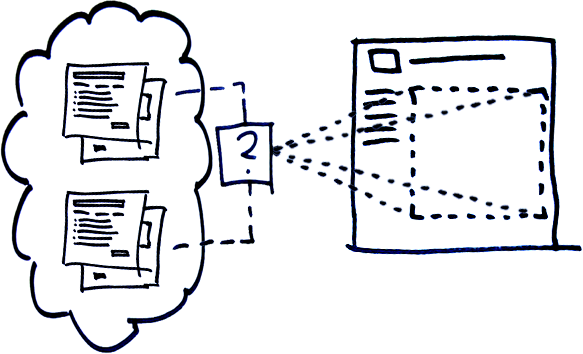
\includegraphics[width=14cm]{skizze.png}
\pagebreak
\section*{Abstract}

Ein Teil der neueren Entwicklung des Internets zum \emph{Web 2.0} basiert auf der Idee, dass Informationen und Funktionen von Software mit Hilfe von \emph{Webservices} verwendet werden können. \cite{hn-web20}

Die Kommunikation mit Webservices ist zwar auf Protokollebene standardisiert, muss jedoch vom Konsumenten immer individuell entsprechend dem Domänenmodell des Anbieters implementiert werden, wodurch eine feste Bindung an den Anbieter entsteht.

Für sogenannte \emph{Blackbox-Webservices} ist das kein Problem --- diese zustandslose Dienste verarbeiten lediglich einfache Daten, d.h. dass der Dienst durch Übergabe eines Datums aufgerufen wird, dieser entsprechend des Aufrufs reagiert und ein Ergebnis zurück liefert.

Anbieter \emph{webbasierter Anwendungen} stehen jedoch vor dem Problem, dass auf Seiten des Anbieters komplexe Arbeitsabläufe abgebildet werden und diese auch persistent innerhalb des Dienstes verbleiben, d.h. sie sind zustandsbehaftet. Auch hier bietet sich die Möglichkeit der Anbindung mittels Schnittstellen, jedoch mit deutlich gesteigertem Aufwand, da zwischen beiden Parteien das Verständnis über die verarbeiteten Entitäten vermittelt werden muss. 

Nach \cite[Seite 653]{ei-sawsdl} sind etablierte Standards für Webservices der ersten Generation wie \acs{SOAP} und \acs{UDDI} primär unter dem Aspekt entwickelt worden, einen einfachen Weg zur Verteilung und Wiederverwertung von Webservices zu etablieren --- ihnen fehlt also eine Standardisierung für das Auffinden, Zusammenstellen und Auswählen von Diensten um eine \emph{lose Kopplung} zu ermöglichen. Für ein lebendiges Web-Öko-System ist die lose Kopplung jedoch von entscheidender Bedeutung --- im Idealfall lassen sich Dienste so anbinden, dass sie jederzeit und ohne Aufwand ausgetauscht werden können und sogar die parallele Verwendung mehrere Dienste der gleichen Art ermöglicht wird.

\textbf{In dieser Seminararbeit möchte ich versuchen die Frage zu beantworten, welche Konzepte für die dynamische Bindung von komplexen Webanwendungen existieren.}

\subsection*{Aufbau dieser Seminararbeit}

Diese Seminar ist unterteilt in acht Abschnitte. Im ersten Abschnitt~(\ref{l:einleitung}) gehe ich auf die Problemstellung~\ref{l:problem} im Detail ein und liefere mehrere Beispiele~(\ref{l:beispiele}) die ich Verlauf der Arbeit immer wieder heran ziehen werde. 

Im zweiten Abschnitt erläutere ich die zu Grunde liegenden Begrifflichkeiten~(\ref{l:definition}). 

Im dritten Abschnitt gehe ich auf die Grundlagen semantischer Webservices ein~(\ref{l:sem-web-ser}).

Im vierten Abschnitt beschreibe ich die gefunden Lösungsansätze~(\ref{l:loesungen}) zu Semantischen~Webservices, die ich im fünften Abschnitt auf ihre Verwendbarkeit für webbasierter Anwendungen~\ref{l:verwendung} analysiere und gebe im sechsten Abschnitt einige reale Beispiele~(\ref{l:sem-web-ser-beispiele}).

Im siebten Abschnitt findet sich das Fazit~(\ref{l:fazit}) und ein Ausblick~(\ref{l:ausblick}) auf zukünftige Auswirkungen und Entwicklungen.

\pagebreak

\tableofcontents

\pagebreak
\section{Einleitung}
\label{l:einleitung}
\subsection{Problemstellung}
\label{l:problem}

Web services generalize the idea of the Web beyond the exchange of simple Web pages in order to enable the provision of a broad range of different services. By composing Web services, cross-organizational and collaborative business processes can be realized in a highly dynamic and flexible way, which is particularly important if services have to be automatically procured at runtime. However, achieving a higher degree of automation is obstructed by the informal nature of legal, contractual and organizational regulations, the numerous and complex service descriptions including manifold customization possibilitiesm and the open and heterogeneous nature of the Web service market.

Because many consider them a server-side activity, the
current development of Web services isn’t requester oriented.
Each service provider has its own business logic and
system design.When the service provider upgrades its system
and architecture to improve the service or add new
service functions, service requesters must change their
applications accordingly. For example, the first version of
ArcWeb Services had no point data type.The location data
type contains the x and y values directly. In the second and
third versions, an application must derive the x and y coordinate
values from the point-object data type. Semantics
become a problem because when providers develop services,
they’re more concerned with the business logic and
how to build the service in OOP.This focus concentrates
on syntactic architecture for service development, not
meaning. Afterward, people find it difficult to have
requesters understand and use services without information
about the underlying meaning behind the services by
reading the WSDL document, the product of OOP. \cite{shi1}

The current Web service technology brought a new potential
to the Web of services. However, the success of Web
services still depends on resolving three fundamental challenges,
namely search, integration and mediation. \cite{WSMOLITE}

\begin{itemize}
\item "Whitebox"-Anbindung
\item Bisher: 1:1-Verbindung (Beispiel Mite)
\item Problem Ontologie. Projekt = Was?
\end{itemize}
\subsection{Beispiele}
\label{l:beispiele}
\begin{itemize}
\item Mite
\item E-Mail-Backup
\end{itemize}
\section{Definition}
\label{l:definition}
\subsection{Webservice}
Anwendungen in Unternehmen werden heute im Gegensatz zu den isolierten Einzellösungen
der Vergangenheitmeist als Aggregate weitgehend eigenständiger Softwarekomponenten realisiert.
Dienstorientierte Architekturen sind die Basis für die Erweiterung dieser Aggregate um
extern erbrachte Dienstkomponenten, die bevorzugt über das Internet als Web Services eingebunden
werden. Damit wird es beispielweise möglich, betriebswirtschaftliche Anwendungen zu
Ablaufketten zu verbinden, externe Informationsdienste in die eigene Planungssoftware einzubeziehen
oder ein netzweites Single-Sign-On zu nutzen. Solche dienstorientierten Architekturen
finden heute große Aufmerksamkeit, weil sich die Anwender dadurch Flexibilität, Interoperabilität,
Anpassungsfähigkeit, Wiederverwendbarkeit, Herstellerunabhängigkeit und letztendlich
Kostenersparnisse für die Entwicklung und den Betrieb der Geschäftsanwendungen erhoffen. \cite{addo}
\subsection{Webservice-Protokolle}
\label{l:wsprot}
\subsection{Blackbox-Dienste}
\label{l:blackbox}
Für die Nutzung eines Dienstes reicht die Kenntnis der Schnittstellen aus. Ein tieferes Verständnis
der internen Vorgänge wird nicht benötigt, bzw. soll bewusst verborgen werden. \cite{hhxmlwssoa}

Beispiele hierfür ist z.B. ein Webservice, der Wetterdaten für eine PLZ liefert. Hier gibt der Konsument die PLZ eines Ortes in Deutschland ein und erhält in der Antwort eine Temperatur. Die genauen technischen Abläufe, wie der Webservice aus der PLZ eine Temperatur ermittelt bleiben für den Konsumenten verborgen und sind für diesen auch irrelevant.

Diese Arten von Diensten sind zustandslos, d.h. sie behandlen jede Anfrage unabhängig von einer vorherigen.
\subsection{Webbasierte Anwendungen, Whitebox-Dienste}
\label{l:webanw}
Nicht zustandslos.

Beispiele hierfür sind z.B. Werkzeuge zur projektspezifischen Zeiterfassung. 
\subsection{Loose Kopplung}
\label{l:loosec}

\section{Semantische (Web-)services}
\label{l:sem-web-ser}
\subsection{Einführung}

Was bleibt ist das Problem der Semantik der auszutauschenden Daten. Deswegen denke ich: Öffentliche Service-Verzeichnisse werden sich im Business-Alltag mangels semantischer Standards vorerst nicht durchsetzen. Viel wahrscheinlicher ist zunächst die Migration bestehender Unternehmensverbände (z.B. Zulieferer - Hersteller, etc.) auf eine Service-orientierte Plattform mit einem gemeinsamen privaten Service-Verzeichnis. Dieses wäre ein weiterer Schritt in Richtung der Vision eines Semantic Web Services bzw. dem Semantic Web.  \cite{hhxmlwssoa} 

Such an approach means service providers handle serialization
and deserialization themselves in the knowledge
engineering process, as Figure 3 shows, rather than using
the computer to do it automatically.So, the service description
becomes meaningful as well as independent of the
OOP development.
Because service semantics can remain consistent for long
periods—despite the changes in system design, business
logic, and APIs—publishing requester-oriented service
semantics is better than publishing the changing APIs specified
in WSDL documents. Most Web service users, including
scientists and engineers, aren’t programmers, so
implementing such requester-oriented service design will
let most users exploit distributed computing’s power without
writing a computer program. \cite{shi1}

\begin{figure}
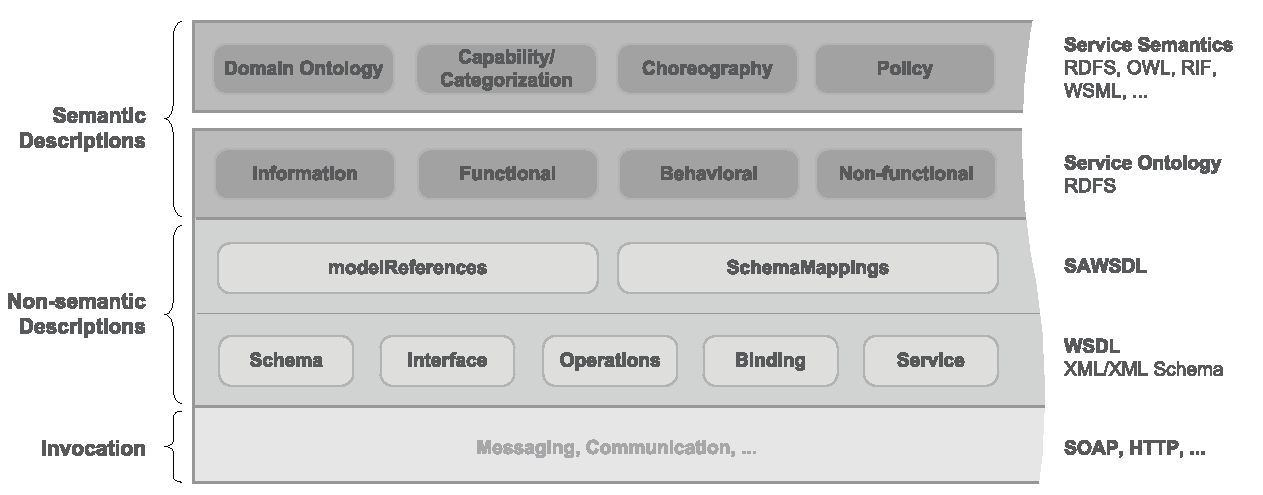
\includegraphics[width=14cm]{Extended-Web-Service-Specification-Stack.pdf}
\caption{Extended Web Service Specification Stack, \cite{WSMOLITE}}
\end{figure}

\subsection{Ontologien}

Das Transportieren von Bedeutung ist Ziel jeder Kommunikation. Dabei
differieren oftmals die gedanklichen Verknüpfungen der verwendeten Worte bei
Sender und Empfänger. In Standard-Situationen, wie zum Beispiel beim
Überqueren einer Fußgängerampel oder in anderen stark reglementierten
Abläufen, besteht kaum Klärungsbedarf hinsichtlich der verwendeten Zeichen
oder des verwendeten Vokabulars. Treffen allerdings Sender und Empfänger in
einem weniger stark reglementierten oder unterschiedliche interpretierbarem
Kontext aufeinander, so müssen zuerst das unterschiedlich verwendete Vokabular
und die dahinterstehenden Bedeutungen abgeglichen werden. [und weiter...] \cite{sgthesis}

\subsection{Ultra Large Scale Systems}

Eine Möglichkeit die Überlebensfähigkeit von digitalen Ökosystemen sicherzustellen
ist es, Redundanz einzuführen und zwar Redundanz auf allen Ebenen, angefangen
von der Hardware über die Betriebssysteme bis hin zur Software und den
eingesetzten Services. Ein solch hohes Maß an Redundanz würde jedoch immense
Investitionen verschlingen, von daher ist es günstiger, mit einer minimalen Redundanz
zu leben und die Qualitäten der gelieferten Services zu reduzieren. Für die
Qualitätsreduktion ist jedoch wichtig zu wissen, was an Services vom System noch
in welcher Qualität zur Verfügung steht und was nicht. Die "überlebenden" Services
werden neu komponiert und den Consumern zur Verfügung gestellt. Diese Form der
ad-hoc Komposition bedingt, dass Servicekomposition (s. Abschn. 2.7.3) sich neben
den fachlichen Interfaces und den "bestmöglichen" Qualitäten auch an Notfallpolicies
orientieren kann. \cite{mkulss}

\section{Lösungsansätze}
\label{l:loesungen}

In this paper we will explore this issue in some detail and we will propose a set of
features that, in our view, will increasingly characterize the Semantic Web
applications. Our analysis aims to be both descriptive and prescriptive. Descriptively,
the objective here is to characterize the space of current Semantic Web applications,
provide dimensions to compare and contrast them, and identify key trends.
Prescriptively, our goal is to specify a number of criteria, which Semantic Web
applications ought to satisfy, if we want to move away from conventional semantic
systems and develop a new generation of Semantic Web applications, which can
succeed in applying semantic technology to the challenging context provided by the
World-Wide-Web. \cite{ngswa}

The current Web service standards around Universal
Description, Discovery and Integration (UDDI) and related technologies do not address this
problem as they offer only service discovery based on attribute/ value queries, that is limited
to atomic service discovery. Research has shown that Business Process Execution Language
for Web Services (BPEL4WS or BPEL for short), which is currently used to express business
processes in Web service environments, does not have a solid formal model and thus lacks
formal semantics for querying business process descriptions. This means that a formal model is
required to express business processes and to enable their querying. Based on this formal model,
appropriate indexing techniques are needed for effcient querying in large service repositories. \cite{mothesis}

\subsection{SAWSDL}

As we noted in section 1, the technology of the Web
services was accompanied by many standards. However,
these standards do not remedy to the problem of adaptability
to Web services’ changes, and do not cover all aspects related
to different tasks of the Web service’s life cycle, namely, the
discovery, the invocation, the publication and the
composition. Indeed, many enterprises applications, in
particular, can constantly have need to discover and use
existing Web services, or to compose them to meet new
requirements or a complex request (eg. a travel agency can
for example use both fly and hotel booking services to
respond a customer’s query). The number of Web services
which increase on Internet makes their discovery and/or
composition a complex task. Automating these tasks is a
solution which would reduce the cost of the Web services’
implementation. Nevertheless, with this intention, we think
that it is necessary to enrich the description of the Web
services by explicit and comprehensible semantics, which can
be used by the machine. \cite{ei-sawsdl}

The more valuable
gain of SAWSDL lies in opportunities to annotate existing
WSDL descriptions in a bottom-up fashion while at the
same time only use descriptions of services which are relevant
to specific domain requirements. \cite{WSMOLITE}

\subsection{ORISF}

This paper presents the Ontology-based Resourceoriented
Information Supported Framework (ORISF). The
framework’s aim is to support RESTful Web Service with
resource model through ontology evolution and RESTful
service description, and realize the semantic-level
integration of resources. \cite{zg-ontorest}

\section{Verwendbarkeit für webbasierter Anwendungen}
\label{l:verwendung}
\section{Beispiele}
\label{l:sem-web-ser-beispiele}
\subsection{Webintents}

\subsection{OpenSearch}

\section{Fazit}
\label{l:fazit}
\section{Ausblick}
\label{l:ausblick}
\pagebreak

\section*{Anhang}
\subsection*{Abkürzungsverzeichnis}
\begin{acronym}
\acro{SOAP}{Simple Object Access Protocol}
\acro{UDDI}{Universal Description, Discovery and Integration}
\end{acronym}

\bibliography{bibliothek}
\end{document}
